\afuncT{clip}{Clip. Computes the generalized double clip of two views. See \cvl{} specification for more information.}{selectionOperations}
\\\cvsiplh
\begin{cfuncs}
void vsip\_mclip\_d(const~vsip\_mview\_d*, vsip\_scalar\_d, vsip\_scalar\_d, vsip\_scalar\_d, vsip\_scalar\_d, const~vsip\_mview\_d*);\Bs\\
void vsip\_mclip\_f(const~vsip\_mview\_f*, vsip\_scalar\_f, vsip\_scalar\_f, vsip\_scalar\_f, vsip\_scalar\_f, const~vsip\_mview\_f*);\Bs\\
void vsip\_mclip\_i(const~vsip\_mview\_i*, vsip\_scalar\_i, vsip\_scalar\_i, vsip\_scalar\_i, vsip\_scalar\_i, const~vsip\_mview\_i*);\Bs\\
void vsip\_mclip\_si(const~vsip\_mview\_si*, vsip\_scalar\_si, vsip\_scalar\_si, vsip\_scalar\_si, vsip\_scalar\_si, const~vsip\_mview\_si*);\Bs\\
void vsip\_vclip\_d(const~vsip\_vview\_d*, vsip\_scalar\_d, vsip\_scalar\_d, vsip\_scalar\_d, vsip\_scalar\_d, const~vsip\_vview\_d*);\Bs\\
void vsip\_vclip\_f(const~vsip\_vview\_f*, vsip\_scalar\_f, vsip\_scalar\_f, vsip\_scalar\_f, vsip\_scalar\_f, const~vsip\_vview\_f*);\Bs\\
void vsip\_vclip\_i(const~vsip\_vview\_i*, vsip\_scalar\_i, vsip\_scalar\_i, vsip\_scalar\_i, vsip\_scalar\_i, const~vsip\_vview\_i*);\Bs\\
void vsip\_vclip\_si(const~vsip\_vview\_si*, vsip\_scalar\_si, vsip\_scalar\_si, vsip\_scalar\_si, vsip\_scalar\_si, const~vsip\_vview\_si*);\Bs\\
void vsip\_vclip\_uc(const~vsip\_vview\_uc*, vsip\_scalar\_uc, vsip\_scalar\_uc, vsip\_scalar\_uc, vsip\_scalar\_uc, const~vsip\_vview\_uc*);\Bs\\
\end{cfuncs}
\pyjvsiph
\viewmthd{No}{NA}{NA}{NA}
%
\apyfunc{Yes}{\ttbf{clip(in,t1,t2,c1,c2,out)}}\\
\hspace*{.08\textwidth}
{\rmfamily For plot of result see figure \ref{fig:ClipExample}.}
\inputminted[linenos=true,resetmargins=true,xleftmargin=.12\textwidth,fontfamily=tt,fontsize=\small]{python}{./pyJvsip_examples/eXclip.py}
\begin{minipage}[c]{\textwidth}\centering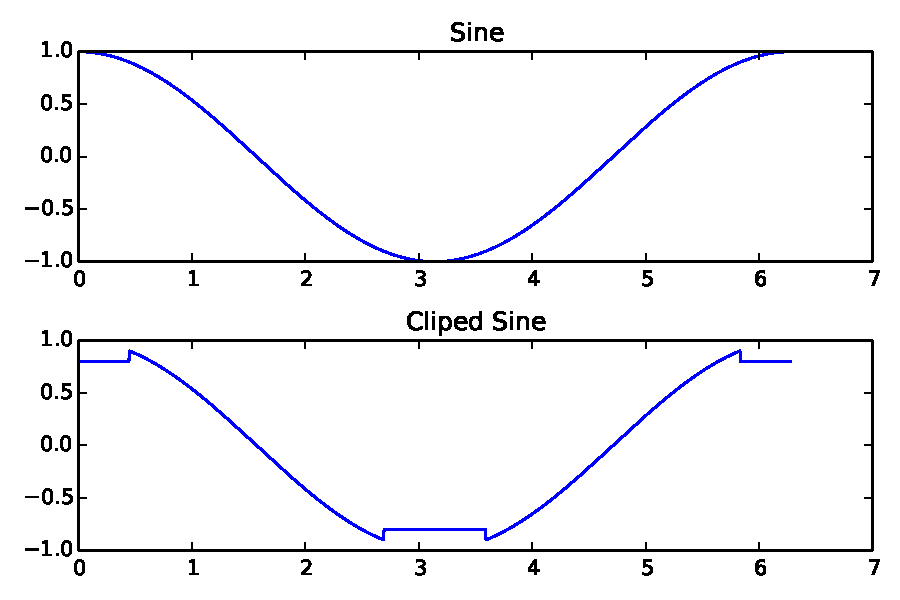
\includegraphics[width=0.8\textwidth]{./pyJvsip_examples/eXclip}\captionof{figure}{Clip Example}
\label{fig:ClipExample}\end{minipage}
\pyComment{
\item{The clip function works much the same as \cvl{} except the output is returned. In line 6 of the example we used the \ttbf{empty} method to create the output vector and saved a reference in the left value.}
\item{The \ttbf{clip} function is a bit complicated. See the \cvl{} specification for more complete details.}
\item{The \ttbf{view} \ttbf{in} is clipped according to the rules of the function. The clipping checks are set by \ttbf{t1} and \ttbf{t2} and the clip values are set by \ttbf{c1} and \ttbf{c2} accordingly. The output is placed in \ttbf{out}. If \ttbf{in==out} then the function is done in-place}
}